\subsection{lag compensation}
$$
G_c(s) = K_c\dfrac{s + \dfrac{1}{T}}{s+\dfrac{1}{\beta T}}, \quad \beta > 1
$$
In lag compensation we find out $K$ for steady state error.
$$K = 5.1300$$
$$\gamma_d = 45^{\circ} \to \bar{\gamma_d} = 45 + 5 = 50^\circ$$
$$
\phi(\omega_g) = 50 - 180 = -130^{\circ}
$$
The phase angle:

$$
\angle G(j\omega) = 0^{\circ} + \tan^{-1}\dfrac{\omega}{0.5} - \tan^{-1}\dfrac{\omega}{1} - 3\tan^{-1}\dfrac{\omega}{1.5} - \tan^{-1}\dfrac{\omega}{2}
$$
$$
\angle G(j\omega_g) = 
0^{\circ} + \tan^{-1}\dfrac{\omega_g}{0.5} - \tan^{-1}\dfrac{\omega_g}{1} - 3\tan^{-1}\dfrac{\omega_g}{1.5} - \tan^{-1}\dfrac{\omega_g}{2} = -130^{\circ}
$$
This equation solved with MATLAB and code has attacked (Q1\_b.m)
$$
\omega_g =  1.2025
$$
The amplitude ratio:
$$
\left\vert G_1(j\omega) \right\vert = \left\vert KG(j\omega) \right\vert = 5.1300\dfrac{50\sqrt{\omega^2+0.5^2}}{\sqrt{\omega^2+1^2}\times(\sqrt{\omega^2 + 1.5^2})^3\times\sqrt{\omega^2 + 2^2}}
$$
$$
\beta = \left\vert G_1(j\omega_g) \right\vert = 
5.1300\dfrac{50\sqrt{\omega_g^2+0.5^2}}{\sqrt{\omega_g^2+1^2}\times(\sqrt{\omega_g^2 + 1.5^2})^3\times\sqrt{\omega_g^2 + 2^2}}
$$

$$
\beta = 5.1300\dfrac{50\sqrt{1.2025^2+0.5^2}}{\sqrt{1.2025^2+1^2}\times(\sqrt{1.2025^2 + 1.5^2})^3\times\sqrt{1.2025^2 + 2^2}} = 12.8807
$$
Assume:
$$
\dfrac{1}{T} = \dfrac{\omega_g}{2} 
\to \dfrac{1}{T}  = 0.6012 \to T = 1.6632
$$
$$
\to \dfrac{1}{\beta T} = 0.0467, \quad K_c = \dfrac{K}{\beta} = \dfrac{5.1300}{12.8807} = 0.3983
$$
$$
G_c(s) = K_c \dfrac{s + \dfrac{1}{T}}{s + \dfrac{1}{\beta T}}
= 0.3983 \dfrac{s + 0.6012}{s + 0.0467}
$$
Bode digram for lag compensation using MATLAB.
\begin{figure}[H]
	\caption{lag compensation Bode digram using MATLAB}
	\centering
	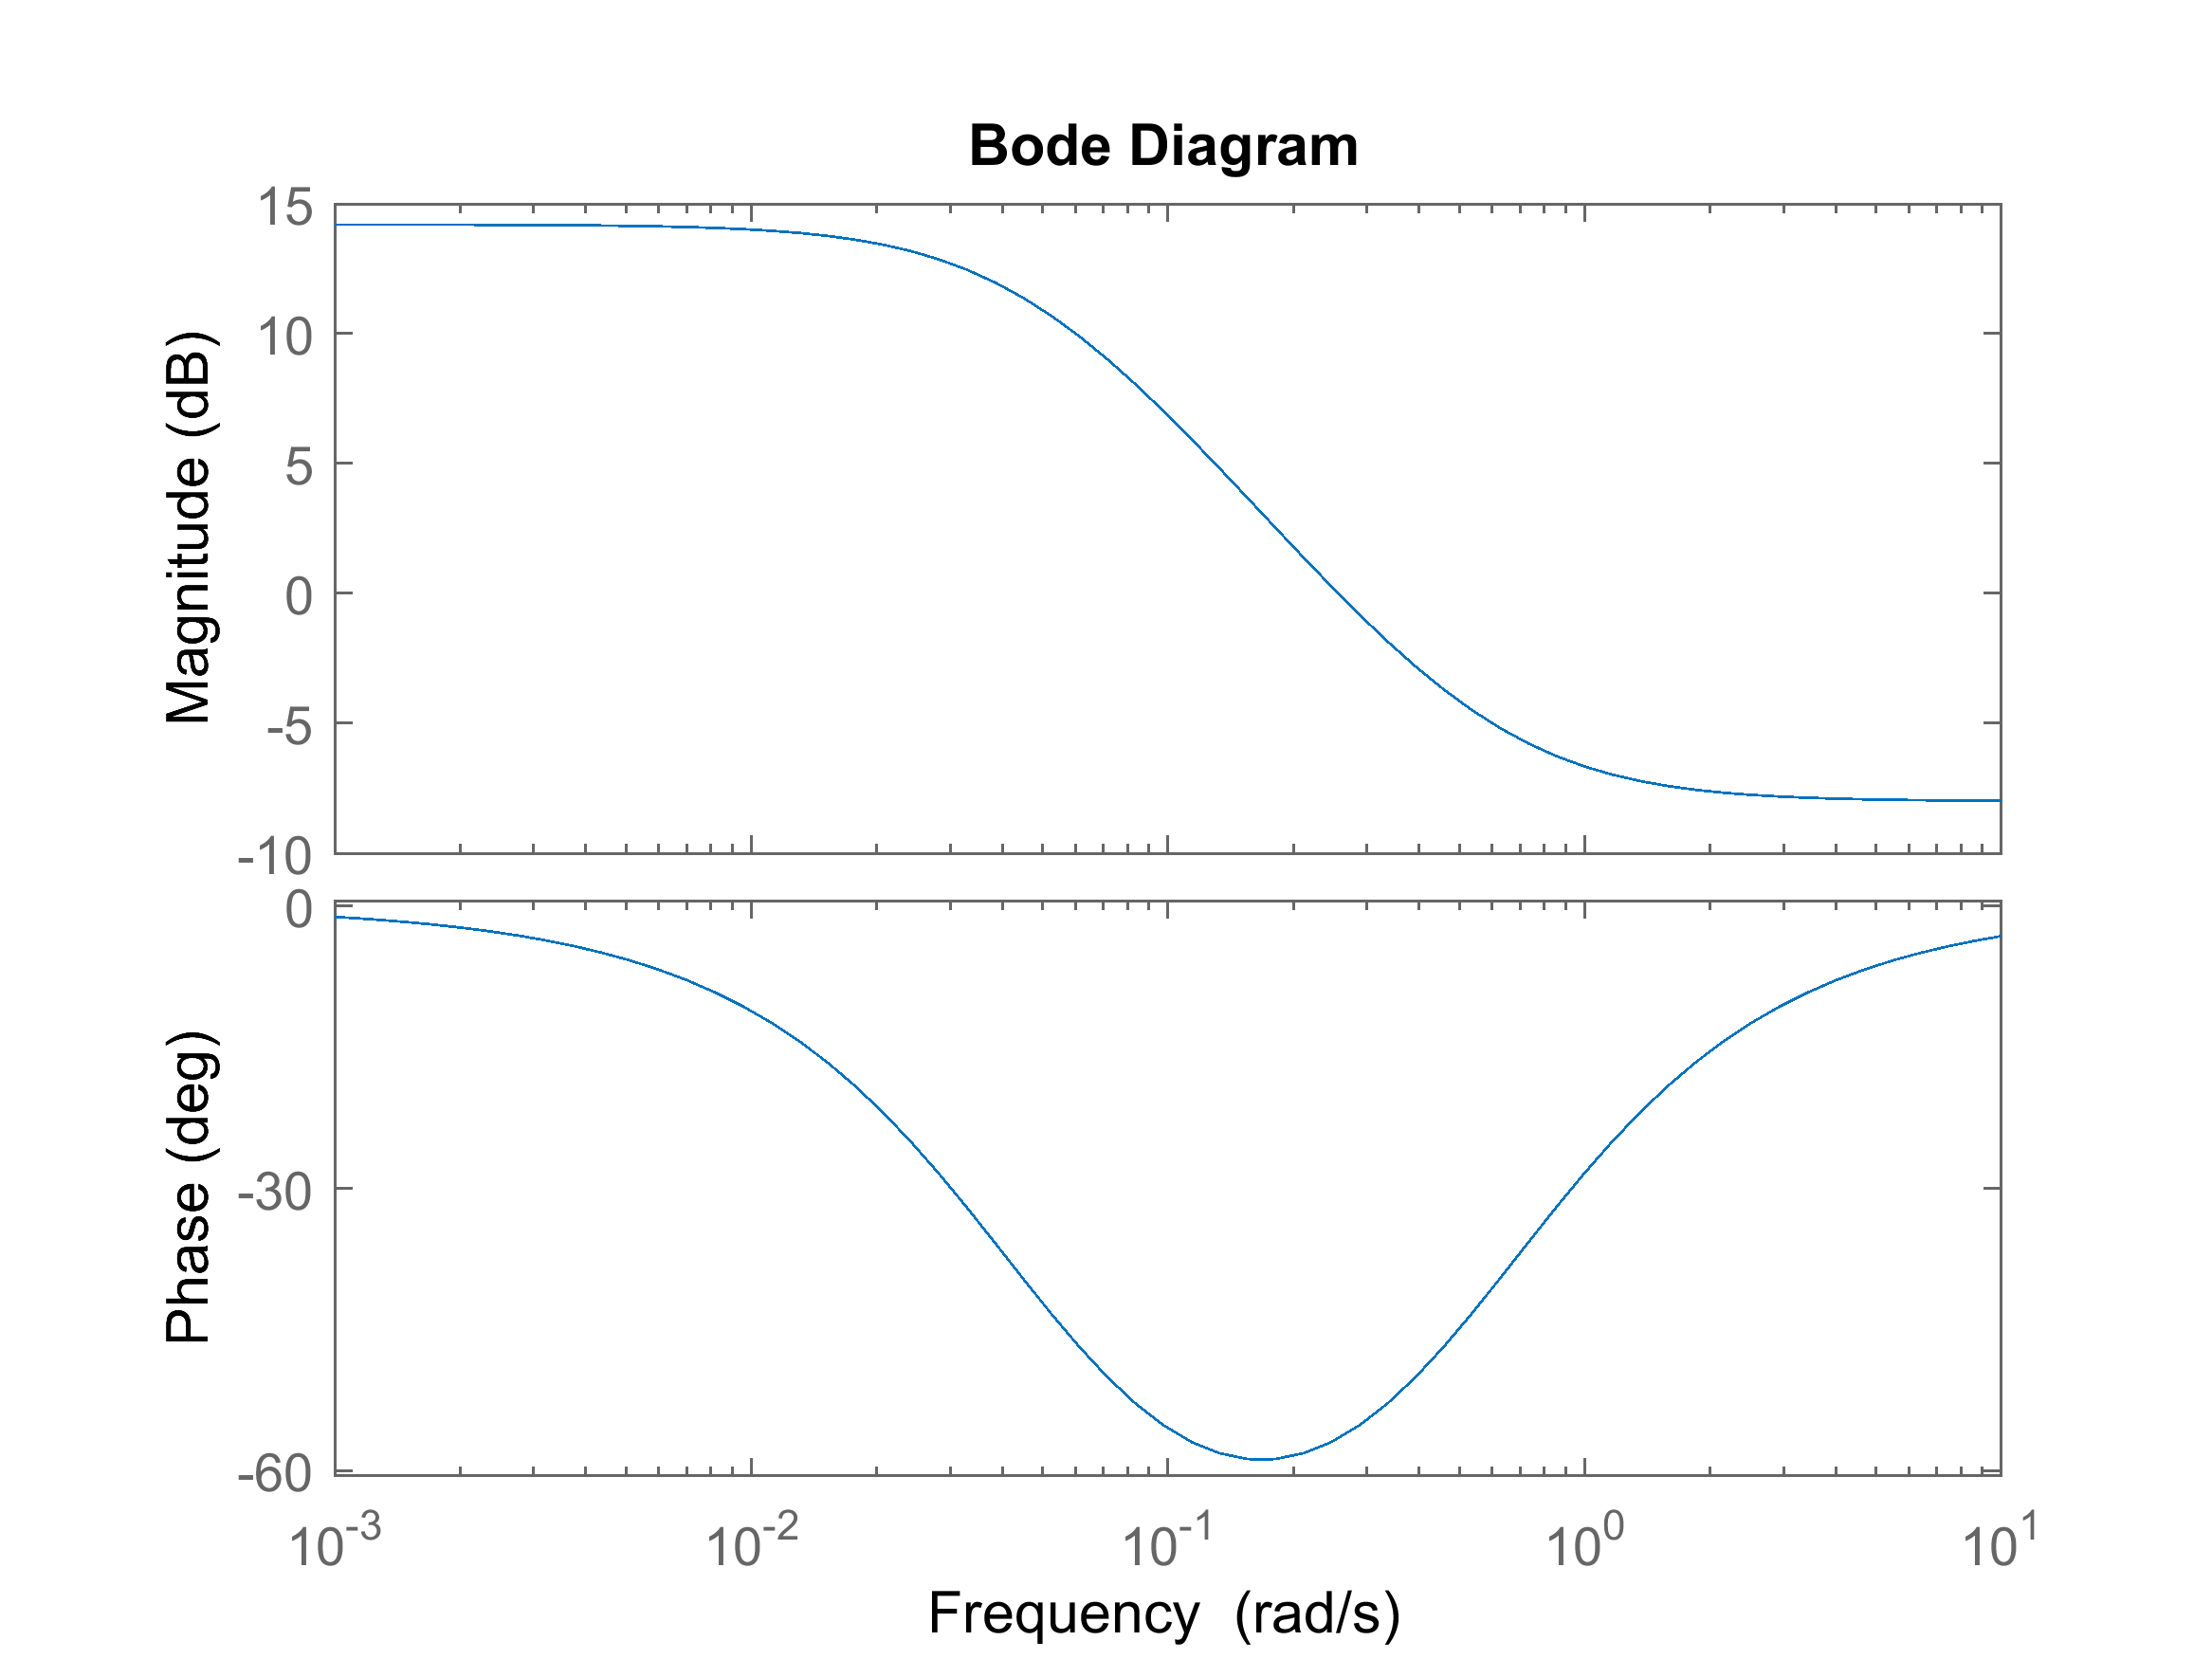
\includegraphics[width=12cm]{../Figure/Q1/b/controller.png}
\end{figure}
Now add lag controller to system.
$$
G_c(s)G(s) = 0.3983 \dfrac{s + 0.6012}{s + 0.0467}\dfrac{50(s+0.5)}{(s+1)(s+1.5)^{3}(s+2)}
$$
Bode digram for system with adding lag compensation.
\begin{figure}[H]
	\caption{Bode digram for system with lag compensation using MATLAB}
	\centering
	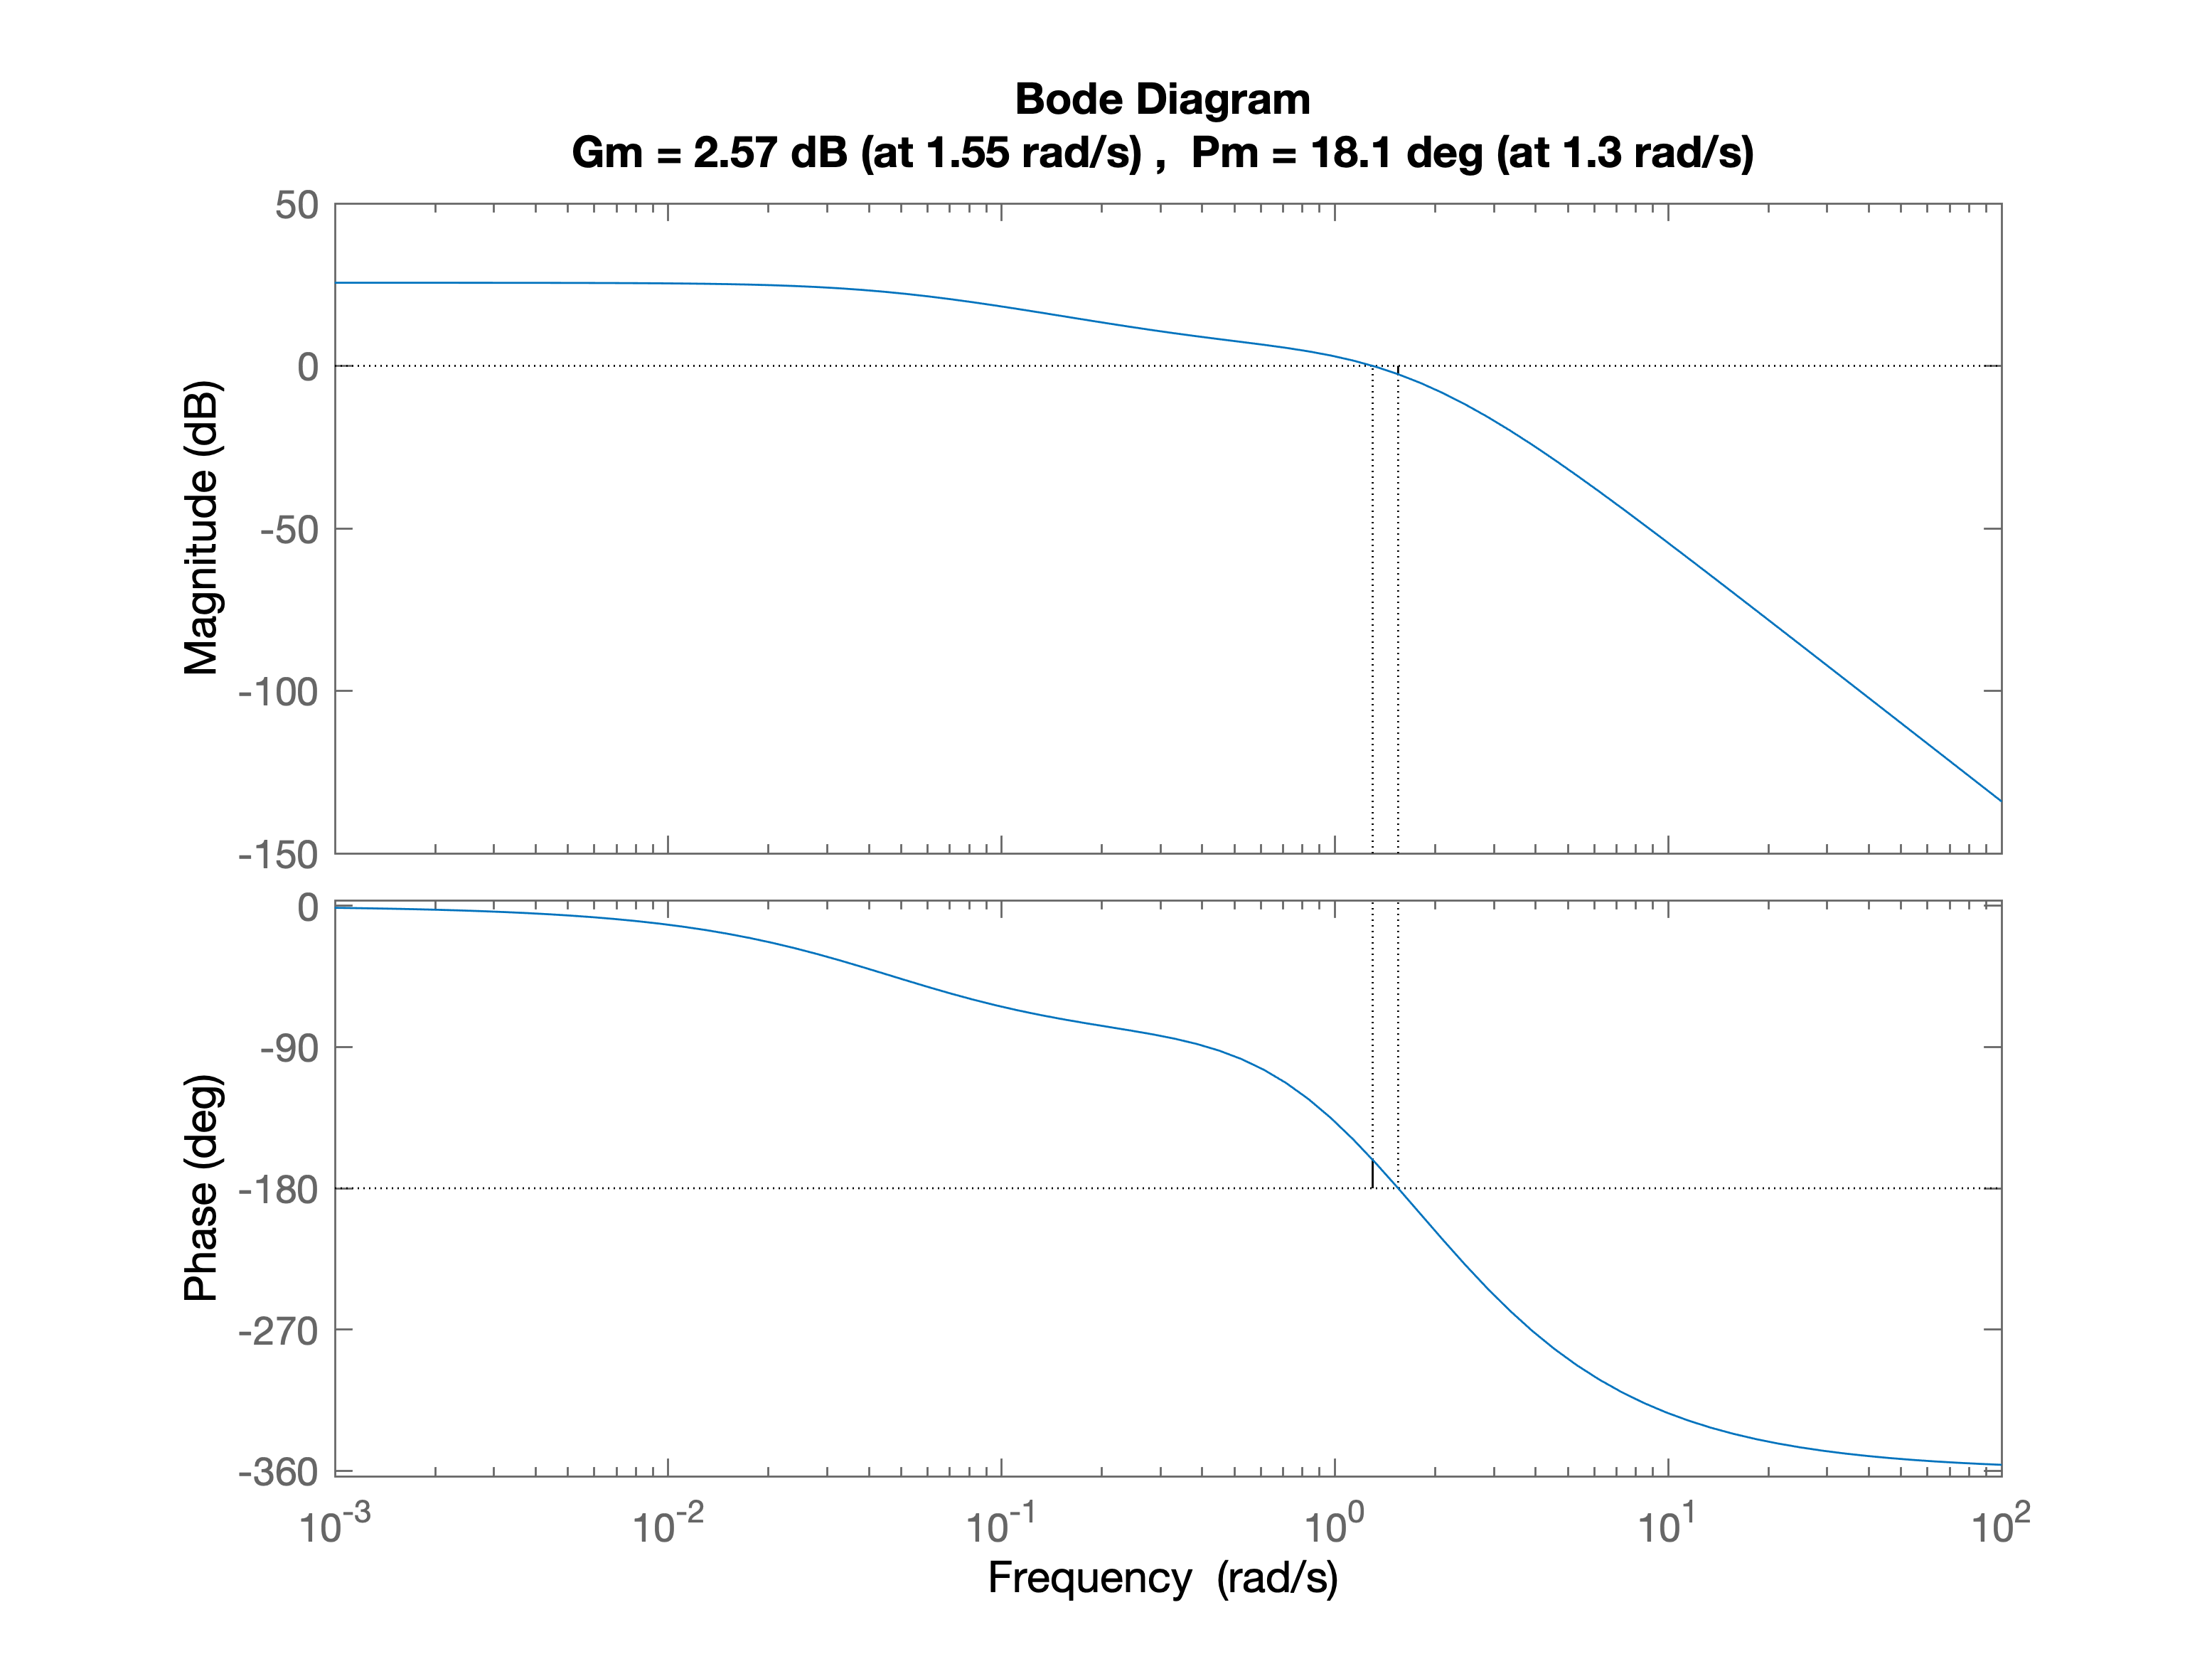
\includegraphics[width=12cm]{../Figure/Q1/b/new_margin.png}
\end{figure}
All bode digram in one figure:
\begin{figure}[H]
	\caption{all bode digram using MATLAB}
	\centering
	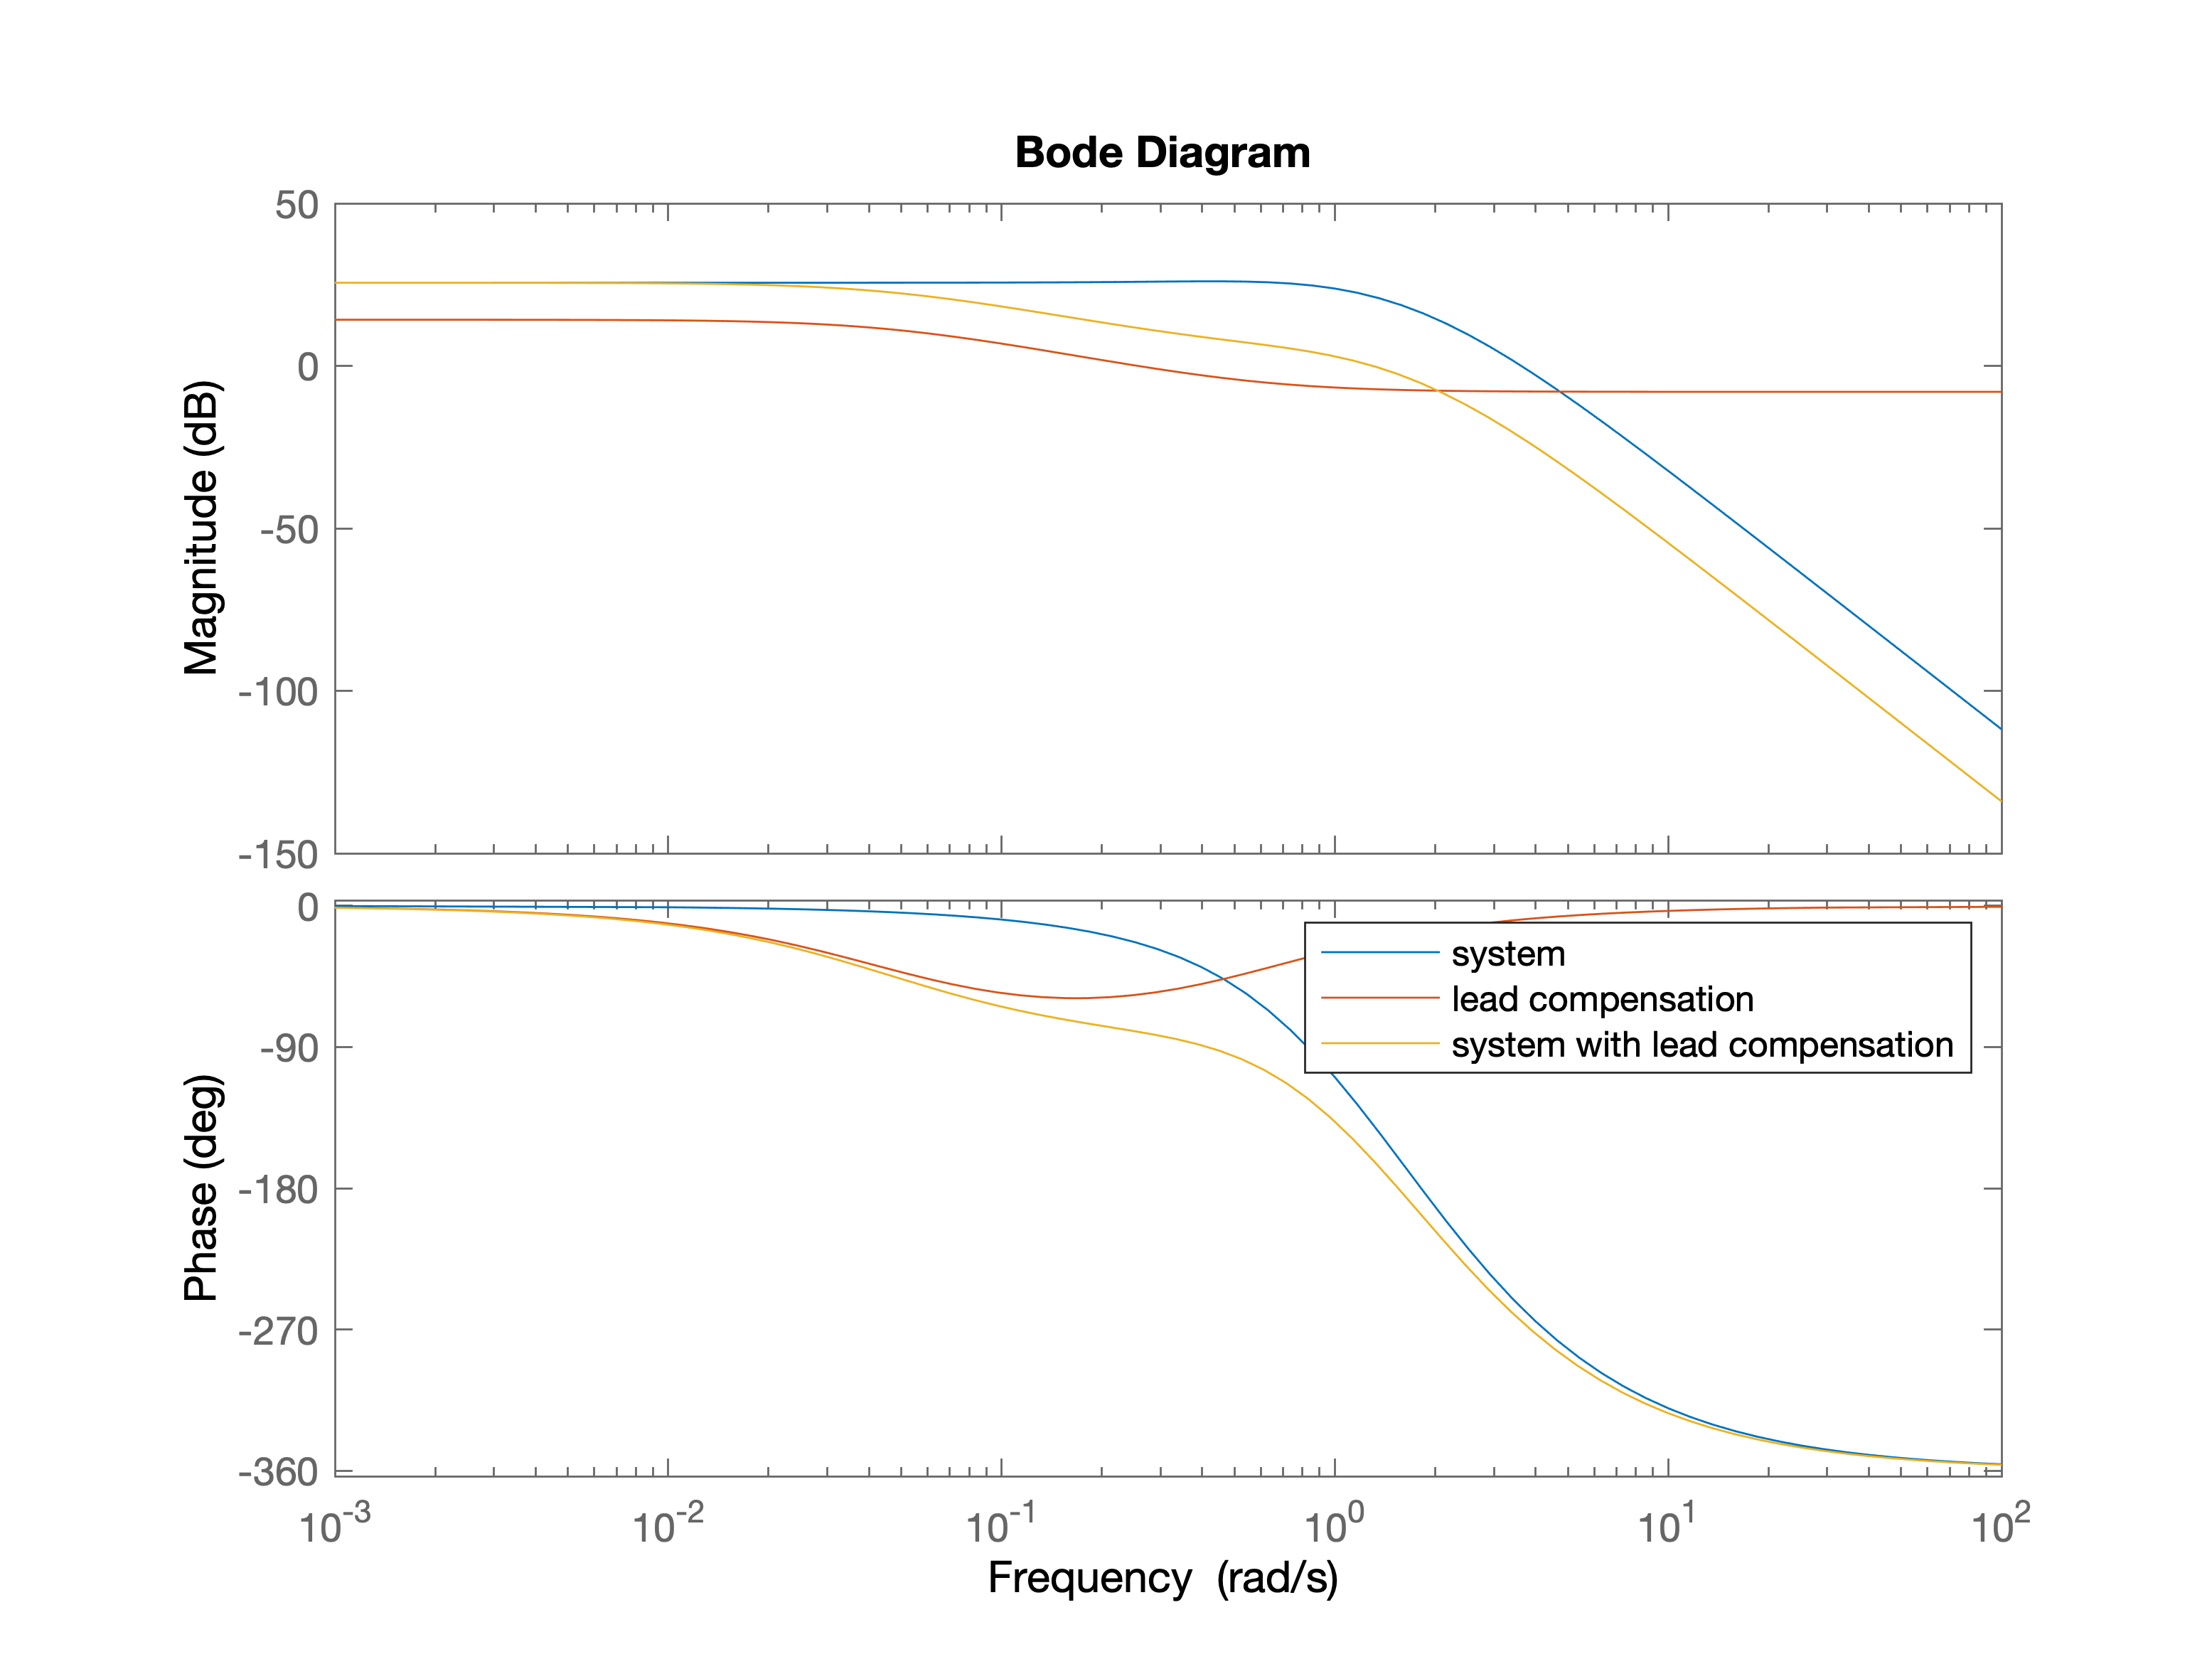
\includegraphics[width=12cm]{../Figure/Q1/b/all_in_one.png}
\end{figure}
We didn't get what we want in equation so we change our before assumation.
assume:
$$
\dfrac{1}{T} = \dfrac{\omega_g}{10} 
\to \dfrac{1}{T}  = 0.1202 \to T = 1.6632
$$
$$
\to \dfrac{1}{\beta T} = 0.0467, \quad K_c = \dfrac{K}{\beta} = \dfrac{5.1300}{12.8807} = 0.3983
$$
$$
G_c(s) = K_c \dfrac{s + \dfrac{1}{T}}{s + \dfrac{1}{\beta T}}
= 0.3983 \dfrac{s + 0.6012}{s + 0.0467}
$$